%%%%%%%%%%%%%%%%%%%%%%% file example.tex %%%%%%%%%%%%%%%%%%%%%%%%%%
%
% This is a template file for the Journal of Physics: Conference Series
%
% Copy it to a new file with a new name and use it as the basis
% for your article
%
%%%%%%%%%%%%%%%%%%%%%%%%%% IOP Publishing %%%%%%%%%%%%%%%%%%%%%%%%%
%

%% The first command in your LaTeX source must be the \documentclass command.
%%
\documentclass[a4paper]{jpconf}

%
% Put here some packages required or/and some personal commands
%
%\usepackage[numbers,sort&compress]{natbib}

\usepackage{amsmath}
\usepackage{hyperref}
\hypersetup{hidelinks}
\usepackage{graphicx}
\usepackage{enumitem}
\usepackage{multirow}

\usepackage{iopams}
\usepackage{cite}
\bibliographystyle{iopart-num-long}   % IOP citation style
%
%% end of the preamble, the start of the body of the document source.
\begin{document}
%
%% The "title" command
\title{How to format your conference paper}
%
% subtitle is optional
%
%%%\subtitle{Do you have a subtitle?\\ If so, write it here}

%% The "author" command and its associated commands are used to define
%% the authors and their affiliations.

%%
%% The "author" command and its associated commands are used to define
%% the authors and their affiliations.
\author{
S O Semerikov$^{1,2,3,4,5}$, 
A E Kiv$^{6,7}$, 
I~S~Mintii$^{8,2,1,3,9,5}$,
T A Vakaliuk$^{3,2,1,5}$, 
P P Nechypurenko$^{1,5}$, 
O~V~Bondarenko$^{1,5}$, 
S L Malchenko$^{1}$,
A~M~Striuk$^{4,1,5}$,
A V Iatsyshin$^{10,11}$, 
V O Artemchuk$^{11,10,12,13}$,
S~V~Klimov$^{14}$, 
H B Danylchuk$^{15}$,
S~M~Chukharev$^{14}$ and
S I Sakhno$^{4}$ 
}

\address{$^{1}$ Kryvyi Rih State Pedagogical University, 54 Universytetskyi Ave., Kryvyi Rih, 50086, Ukraine}
\address{$^{2}$ Institute for Digitalisation of Education of the NAES of Ukraine, 9 M.~Berlynskoho Str., Kyiv, 04060, Ukraine}
\address{$^{3}$ Zhytomyr Polytechnic State University, 103 Chudnivska Str., Zhytomyr, 10005, Ukraine}
\address{$^{4}$ Kryvyi Rih National University, 11 Vitalii Matusevych Str., Kryvyi Rih, 50027, Ukraine}
\address{$^{5}$ Academy of Cognitive and Natural Sciences, 54 Universytetskyi Ave., Kryvyi Rih, 50086, Ukraine}
\address{$^{6}$ South Ukrainian National Pedagogical University named after K. D. Ushynsky, 26~Staroportofrankivska Str., Odesa, 65020, Ukraine}
\address{$^{7}$ Ben-Gurion University of the Negev, P.O.B. 653, Beer Sheva, 8410501, Israel}
\address{$^{8}$ University of Łódź, 68 Gabriela Narutowicza Str., 90-136 Łódź, Poland}
\address{$^{9}$ Lviv Polytechnic National University, 12 Stepana Bandery Str., Lviv, 79000, Ukraine}
\address{$^{10}$ Center for Information-analytical and Technical Support of Nuclear Power Facilities Monitoring of the NAS of Ukraine, 34a Palladin Ave., Kyiv, 03142, Ukraine}
\address{$^{11}$ G.E. Pukhov Institute for Modelling in Energy Engineering of the NAS of Ukraine, 15~General Naumov Str., Kyiv, 03164, Ukraine}
\address{$^{12}$ National Aviation University, 1 Liubomyra Huzara Ave., Kyiv, 03058, Ukraine}
\address{$^{13}$ Kyiv National Economic University named after Vadym Hetman, 54/1 Beresteiskyi Ave., Kyiv, 03057, Ukraine}
\address{$^{14}$ National University of Water and Environmental Engineering, 11 Soborna Str., Rivne, 33028, Ukraine}
\address{$^{15}$ The Bohdan Khmelnytsky National University of Cherkasy, 81 Shevchenko Blvd., Cherkasy, 18031, Ukraine}


\ead{
semerikov@gmail.com, 
kiv.arnold20@gmail.com,
irina.mintiy@kdpu.edu.ua,
tetianavakaliuk@gmail.com,   
acinonyxleo@gmail.com, 
bondarenko.olga@kdpu.edu.ua,
malchenko.svitlana@kdpu.edu.ua,
andrey.n.stryuk@gmail.com,
iatsyshyn.andriy@gmail.com, 
ak24avo@gmail.com,
s.v.klimov@nuwm.edu.ua, 
abdanilchuk@gmail.com,
konf.knu2@gmail.com, 
budfac@gmail.com
}


%% The abstract is a summary of the work to be presented in the
%% article.
\begin{abstract}
This article provides a detailed guide on formatting papers for publication in \iopp\ journals. Based on the ``jpconf'' document class, it offers an overview of the essential formatting elements and common variations authors should utilize when preparing their manuscripts. The paper covers aspects such as structuring the document, formatting text and equations, inserting figures and tables, and managing citations and references using \BibTeX{}. Additionally, it provides best practices for exporting citations. This guide aims to streamline the submission process, enhance the quality of manuscripts, and ensure compliance with \iopp{} standards. By following these instructions, authors can improve their chances of successful publication and contribute to the efficiency of the peer review and publishing process.\footnote{An article abstract should not normally exceed 200 words in a single paragraph. This template does not use any keywords.}
\end{abstract}
%

\section{On the \LaTeX}

Working on past proceedings led the editorial board closer to the idea that it is easier to reject a poorly formatted article rather than spend time editing it and delaying the publication of the complete proceedings volume. As a result, authors are highly recommended to read this handbook from beginning to end before beginning work on their piece. Failure to follow the formatting guidelines will result in the article being rejected at the review stage or even sooner.

Traditionally, we use \LaTeX{} templates for the conference proceedings for many reasons, the main of them being the attempt to decrease the extra amount of editing efforts for the proceedings editors. You can freely use any \LaTeX{} compatible typesetting system (e.g., TeXstudio + TeX Live is a good choice for any operating system). However, if you do not want to be involved in the \LaTeX{} system administration, we propose using a cloud-based \LaTeX{} editor like Overleaf.
After registering at \url{https://www.overleaf.com}, you can start your paper revision with this template using the ``New Project'' -- ``Upload Project'' menu (\fref{fig1}).

\begin{figure}[h]
\centering
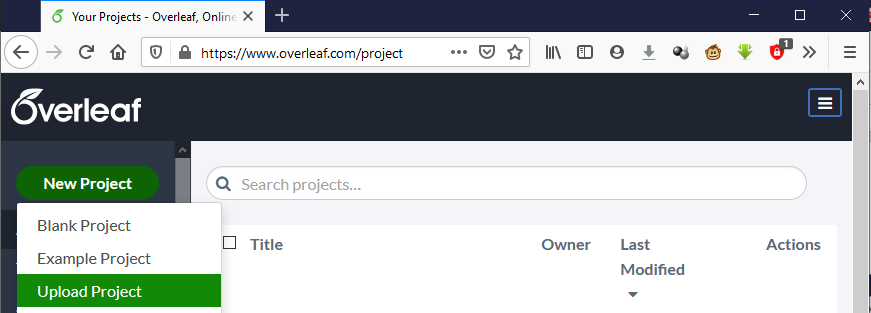
\includegraphics[width=\linewidth]{img/overleaf_1}
\caption{How to upload your project to Overleaf, part 1.}
\label{fig1}       % Give a unique label
\end{figure}

The next step is to select the template archive -- you can download it from the conference website (\fref{fig2}, \fref{fig3}). Alternatively, you can use an online template in Overleaf provided on the conference website.


\begin{figure}[h]
\centering
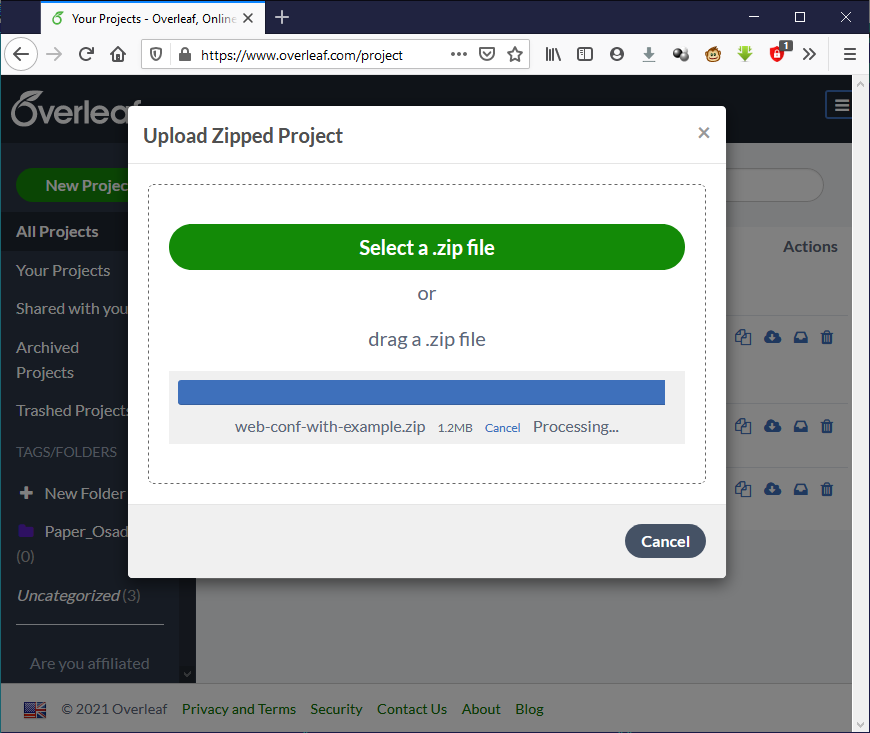
\includegraphics[width=\linewidth]{img/overleaf_2}
\caption{How to upload your project to Overleaf, part 2.}
\label{fig2}       % Give a unique label
\end{figure}


\begin{figure}[h]
\centering
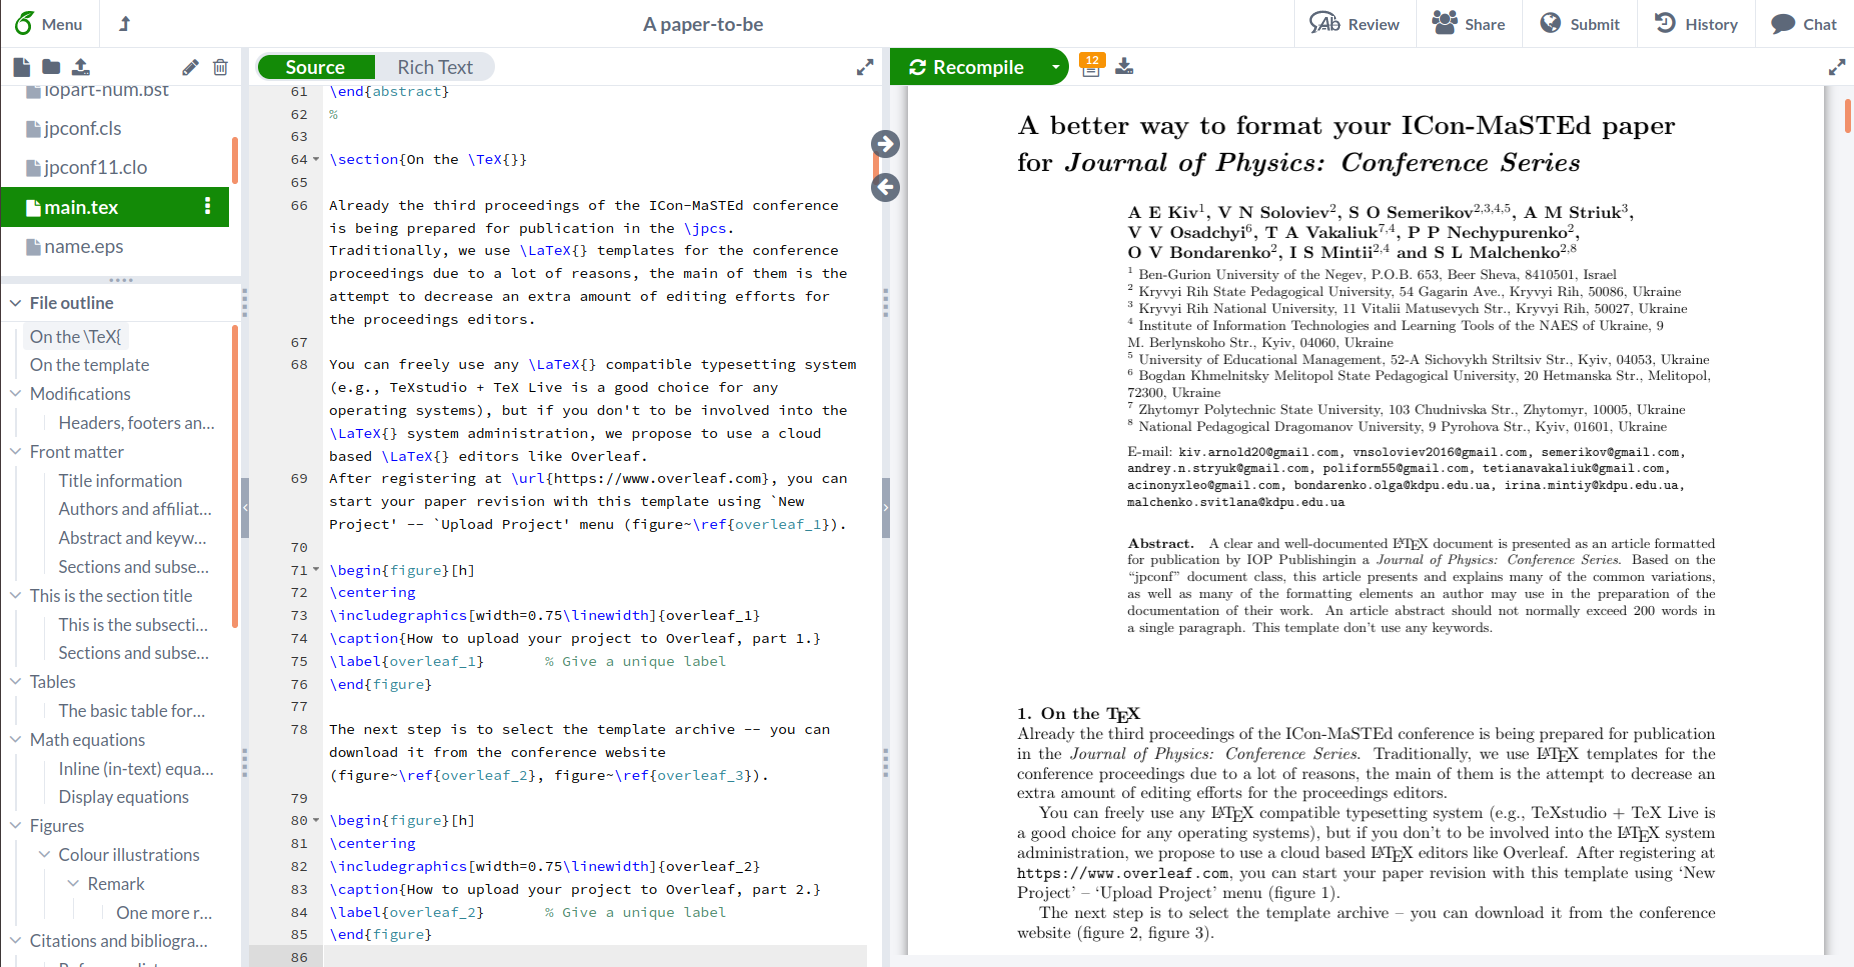
\includegraphics[width=\linewidth]{img/overleaf_3}
\caption{Overleaf, online \LaTeX{} editor.}
\label{fig3}       % Give a unique label
\end{figure}

To get a camera-ready version of your paper in PDF, you can click on the ``Download PDF'' icon or use ``Menu'' to download both LaTeX source files (ZIP) and the camera-ready version (PDF) (\fref{fig4}).

\begin{figure}[h]
\centering
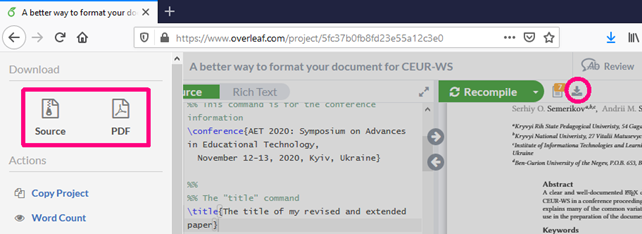
\includegraphics[width=\linewidth]{img/overleaf_4}
\caption{How to download your project from Overleaf.}
\label{fig4}       % Give a unique label
\end{figure}


The most often recommended tutorials are ``The (Not So) Short Introduction to \LaTeX{}2$\varepsilon$''. (\url{https://www.ctan.org/tex-archive/info/lshort/}) and ``Learn LaTeX in 30 minutes''  (\url{https://www.overleaf.com/learn/latex/Learn_LaTeX_in_30_minutes}).

\section{On the template}

\verb"jpconf" requires \LaTeXe\ and can be used with other package files such as those loading the AMS extension fonts \verb"msam" and \verb"msbm" (these fonts provide the blackboard bold alphabet and various extra maths symbols as well as symbols useful in figure captions); an extra style file \verb"iopams.sty" is provided to load these packages and provide extra definitions for bold Greek letters. 

The \verb"iopart-num-long" \BibTeX{} style is intended for use in preparing manuscripts for Institute of Physics Publishing (\iopp{}) journals, including \jpcs{} and \textit{IOP~Conference Series: Earth and Environmental Science}. It provides numeric citations with Harvard-like formatting. We recommend using an updated version of this style with DOI support.

If you are new to publishing with \iopp{} journals, this document is a valuable guide to the process of preparing your work for publication.

To begin the use of the template, you need to:

\begin{enumerate}[label=\arabic*.]
 \item Download and unpack \LaTeX{} template  \url{http://cms.iopscience.iop.org/alfresco/d/d/workspace/SpacesStore/a83f1ab6-cd8f-11e0-be51-5d01ae4695ed/LaTeXTemplates.zip}
 \item Download and unpack \BibTeX{} style  \url{https://github.com/ssemerikov/iopart-num/archive/refs/heads/master.zip}
 \item Copy \verb|jpconf.cls| and \verb|jpconf11.clo| from unpacked \verb|LaTeXTemplates.zip|, and \verb|iopams.sty| and \verb|iopart-num-long.bst| from unpacked \verb|master.zip| to a place where \LaTeX{} can find them or copy them in the same directory as the source file of the article.
\end{enumerate}


\section{Modifications}

Modifying the template -- including but not limited to adjusting margins, typeface sizes, line spacing, paragraph and list definitions, and the use of the \verb|\vspace| command to adjust the vertical spacing between elements of your work manually -- is not allowed.

\subsection{Headers, footers and page numbers}
Authors should {\it not} add headers, footers or page numbers to the pages of their article -- they will be added by \iopp\ as part of the production process.


\section{Front matter}
\label{fpage}

\subsection{Title information}

The titles of papers should all use the regular English style: the first letter of the title should be capitalized with the rest in lowercase. Use the \verb|title| command to define the title of your work. Do not
insert line breaks in your title.
\begin{verbatim}
\title{A better way to format your document for the conference}
\end{verbatim}

Do \textit{not} use any capitalization like ``A BETTER WAY TO FORMAT YOUR DOCUMENT FOR THE CONFERENCE'' or ``A Better Way to Format Your Document for the Conference'' -- both of them are inappropriate.


\subsection{Authors and affiliations}

The following information is required: the list of all authors' names followed by their affiliations. For the authors' names, type \verb"\author{#1}",  where \verb"#1" is the list of all authors' names. The style for the names is initials then surname, with a comma after all but the last two names, which are separated by ``and''. Initials should {\it not} have 
full stops. Feel free to use a tilde sign (\verb"~") for non-breaking space between initials and surname. 

The correct style for the name ``Serhiy O. Semerikov'' is ``S O Semerikov'' only, \textit{not} ``S.~O.~Semerikov''.

The addresses of the authors' affiliations follow the list of authors. Each address should be set by using \verb"\address{#1}" with the address as the single parameter in braces.  If there is more than one address, then a superscripted number, followed by a space, should appear at the start of each address. In this case, each author should also have a superscripted number or numbers following their name to indicate which address is appropriate for them.

Please ensure that affiliations are as complete as possible and include the department, institution, full postal address, postal index, and country. If the authors are at different addresses, numbered superscripts should be used after each surname to reference an author to his/her address.
Multiple authors may share one affiliation. 

Please also provide e-mail addresses for any or all of the authors using an \verb"\ead{#1}" command after the last address. \verb"\ead{#1}" provides the text E-mail: so \verb"#1" is just the e-mail address or a list of e-mails.  

\begin{verbatim}
\author{
	S O Semerikov$^{1,2,3,4,5}$, 
	A E Kiv$^{6,7}$, 
	I~S~Mintii$^{8,2,1,3,9,5}$,
	T A Vakaliuk$^{3,2,1,5}$, 
	P P Nechypurenko$^{1,5}$, 
	O~V~Bondarenko$^{1,5}$, 
	S L Malchenko$^{1}$,
	A~M~Striuk$^{4,1,5}$,
	A V Iatsyshin$^{10,11}$, 
	V O Artemchuk$^{11,10,12,13}$,
	S~V~Klimov$^{14}$, 
	H B Danylchuk$^{15}$,
	S~M~Chukharev$^{14}$ and
	S I Sakhno$^{4}$ 
}

\address{$^{1}$ Kryvyi Rih State Pedagogical University, 
                54 Universytetskyi Ave., Kryvyi Rih, 50086, Ukraine}
\address{$^{2}$ Institute for Digitalisation of Education of the NAES of Ukraine, 
	                9 M.~Berlynskoho Str., Kyiv, 04060, Ukraine}
\address{$^{3}$ Zhytomyr Polytechnic State University, 
	                103 Chudnivska Str., Zhytomyr, 10005, Ukraine}
\address{$^{4}$ Kryvyi Rih National University, 
	                11 Vitalii Matusevych Str., Kryvyi Rih, 50027, Ukraine}
\address{$^{5}$ Academy of Cognitive and Natural Sciences, 
	                54 Universytetskyi Ave., Kryvyi Rih, 50086, Ukraine}
\address{$^{6}$ South Ukrainian National Pedagogical University named after 
	                K. D. Ushynsky, 26 Staroportofrankivska Str., Odesa, 65020, Ukraine}
\address{$^{7}$ Ben-Gurion University of the Negev, 
	                P.O.B. 653, Beer Sheva, 8410501, Israel}
\address{$^{8}$ University of Łódź, 
	                68 Gabriela Narutowicza Str., 90-136 Łódź, Poland}
\address{$^{9}$ Lviv Polytechnic National University, 
	                12 Stepana Bandery Str., Lviv, 79000, Ukraine}
\address{$^{10}$ Center for Information-analytical and Technical Support of 
	                Nuclear Power Facilities Monitoring of the NAS of Ukraine, 
	                34a Palladin Ave., Kyiv, 03142, Ukraine}
\address{$^{11}$ G.E. Pukhov Institute for Modelling in Energy Engineering 
	                of the NAS of Ukraine, 15 General Naumov Str., Kyiv, 03164, Ukraine}
\address{$^{12}$ National Aviation University, 
	                1 Liubomyra Huzara Ave., Kyiv, 03058, Ukraine}
\address{$^{13}$ Kyiv National Economic University named after Vadym Hetman, 
	                54/1 Beresteiskyi Ave., Kyiv, 03057, Ukraine}
\address{$^{14}$ National University of Water and Environmental Engineering, 
	                11 Soborna Str., Rivne, 33028, Ukraine}
\address{$^{15}$ The Bohdan Khmelnytsky National University of Cherkasy, 
	                81 Shevchenko Blvd., Cherkasy, 18031, Ukraine}


\ead{
	semerikov@gmail.com, 
	kiv.arnold20@gmail.com,
	irina.mintiy@kdpu.edu.ua,
	tetianavakaliuk@gmail.com,   
	acinonyxleo@gmail.com, 
	bondarenko.olga@kdpu.edu.ua,
	malchenko.svitlana@kdpu.edu.ua,
	andrey.n.stryuk@gmail.com,
	iatsyshyn.andriy@gmail.com, 
	ak24avo@gmail.com,
	s.v.klimov@nuwm.edu.ua, 
	abdanilchuk@gmail.com,
	konf.knu2@gmail.com, 
	budfac@gmail.com, 
}
\end{verbatim}


\subsection{Abstract and keywords}

The abstract follows the addresses and should give readers concise information about the content of the article and should not typically exceed 200 words. {\bf All articles must include an abstract}. To indicate the start of the abstract, type \verb"\begin{abstract}" followed by the text of the abstract. The abstract should normally be restricted 
to a single paragraph and is terminated by the command
\verb"\end{abstract}".

\begin{verbatim}
\begin{abstract}
  This is an abstract.
\end{abstract}
\end{verbatim}

Do \textit{not} enter keywords for this journal.

The command \verb"\maketitle" is not required.

\subsection{Sections and subsections}\label{subsection}

\begin{verbatim}
\section{This is the section title}
\subsection{This is the subsection title}\label{subsection}
\end{verbatim}

Cross-references to other sections in the text should be made using labels (\sref{subsection})  but can also be made manually.

\begin{verbatim}
\subsection{Sections and subsections \label{subsection}}
\end{verbatim}

\section{Tables}

Tables should be numbered sequentially throughout the text and referred to in the text by number (table 1, etc., {\bf rather than} tab. 1). Each table should be a float and be positioned within the text at the most convenient place near to where it is first mentioned in the text. It should have an explanatory caption that is as concise as possible. Captions should be placed at the top of the table and should have a full stop (period) at the end. 

\subsection{The basic table format}
The standard form for a table is:
\begin{verbatim}
\begin{table}
\caption{Table caption.}
\label{tab1}
\centering
\begin{tabular}{llll}
\br
Head 1&Head 2&Head 3&Head 4\\
\mr
1.1&1.2&1.3&1.4\\
2.1&2.2&2.3&2.4\\
\br
\end{tabular}
\end{table}
\end{verbatim}

The above code produces \tref{tab1}.

\begin{table}[h]
\caption{Table caption.}
\label{tab1}
\centering
\begin{tabular}{llll}
\br
Head 1&Head 2&Head 3&Head 4\\
\mr
1.1&1.2&1.3&1.4\\
2.1&2.2&2.3&2.4\\
\br
\end{tabular}
\end{table}

Points to note are:

\begin{enumerate}[label=\arabic*.]
\item The caption comes before the table.

\item The regular style is for tables to be centred in the same way as equations. This is accomplished by using \verb"\centering".

\item The default alignment of columns should be aligned left.

\item Tables should have only horizontal rules and no vertical ones. The rules at the top and bottom are thicker than internal rules and are set with \verb"\br" (bold rule). The rule separating the headings from the entries is set with \verb"\mr" (medium rule). These commands do not need a following double backslash.

\item Numbers in columns should be aligned as appropriate, usually on the decimal point; to help do this, a control sequence \verb"\lineup" has been defined which sets \verb"\0" equal to a space the size of a digit, \verb"\m" to be a space the width of a minus sign, and \verb"\-" to be a left overlapping minus sign. \verb"\-" is for use in text mode, while the other two commands may be used in maths or text. (\verb"\lineup" should only be used within a table environment after the caption so that \verb"\-" has its normal meaning elsewhere.) See \tref{tab2} for an example of a table where \verb"\lineup" has been used.
\end{enumerate}

\begin{table}[h]
\caption{\label{tab2}A simple example produced using the standard table commands  and $\backslash${\tt lineup} to assist in aligning columns on the decimal point. The width of the table and rules is set automatically by the 
preamble.} 
\centering

\lineup
\begin{tabular}{*{7}{l}}
\br                              
$\0\0A$&$B$&$C$&\m$D$&\m$E$&$F$&$\0G$\\
\mr
\0\023.5&60  &0.53&$-20.2$&$-0.22$ &\01.7&\014.5\\
\0\039.7&\-60&0.74&$-51.9$&$-0.208$&47.2 &146\\
\0123.7 &\00 &0.75&$-57.2$&\m--   &--  &--\\ 
3241.56 &60  &0.60&$-48.1$&$-0.29$ &41   &\015\\ 
\br
\end{tabular}
\end{table}

You can find a lot of examples at \href{https://www.overleaf.com/learn/latex/Tables}{\textit{Overleaf documentation on tables}}. 

\section{Math equations}

You may want to display math equations in three distinct styles: inline, numbered or non-numbered display. Each of the three are discussed in the next sections.

Equations may be numbered sequentially throughout the text (i.e., (1), (2), (3), ...) or numbered by section (i.e., (1.1), (1.2), (2.1), ...) depending on the author’s personal preference. In articles with several appendices, equation numbering by section is useful in the appendices even when sequential numbering has been used throughout the main body of the text: for example,  A.1, A.2 and so forth. When referring to an equation in the text, always put the equation number in brackets -- e.g. ‘as in equation (2)’ or ‘as in equation (2.1)’ -- and always spell out the word ‘equation’  in full, e.g. ‘if equation (5) is factorized’; do not use abbreviations such as ‘eqn.’ or ‘eq.’.

\subsection{Inline (in-text) equations}

A formula that appears in the running text is called an inline or in-text formula. It is produced by the \verb|math| environment, which can be invoked with the usual \verb|\begin| \ldots \verb|\end| construction or with the short form \verb|$| \ldots \verb|$|. You can use any of the symbols and structures, from $\alpha$ to $\omega$; this section will show a few examples of in-text equations in context. Notice how this equation:
\begin{math}
\lim\limits_{n\rightarrow \infty} \frac{1}{n} = 0,
\end{math}
set here in in-line math style, looks slightly different when set in display style (see next subsection).

\subsection{Display equations}

A numbered display equation -- one set off by vertical space from the text and centred horizontally -- is produced by the \verb|equation| environment. An unnumbered display equation is produced by the \verb|displaymath| environment (or \verb|equation*| with \verb|amsmath| package).

Again, in either environment, you can use any of the symbols and structures available in \LaTeX{}; this section will give a couple of examples of display equations in context. First, consider the equation shown as an inline equation above:
\begin{verbatim}
\begin{equation}
\lim_{n\rightarrow \infty} \frac{1}{n} = 0.
\end{equation}
\end{verbatim}
\begin{equation}
\lim_{n\rightarrow \infty} \frac{1}{n} = 0.
\end{equation}

Notice how it is formatted somewhat differently in
the \verb|displaymath| environment. Now, we will enter an unnumbered equation:
\begin{verbatim}
\begin{displaymath}
S_{n} = \sum_{i=1}^{n} x_{i} ,
\end{displaymath}
\end{verbatim}
\begin{displaymath}
S_{n} = \sum_{i=1}^{n} x_{i} ,
\end{displaymath}
and follow it with another numbered equation:
\begin{verbatim}
\begin{equation}\label{lim}
\lim_{x \to 0} (1 + x)^{1/x} = e
\end{equation}
\end{verbatim}
\begin{equation}\label{lim}
\lim_{x \to 0} (1 + x)^{1/x} = e
\end{equation}
to demonstrate \LaTeX's able handling of numbering.

Usually, equations should be centred and should be numbered with the number on the right-hand side. (You can find additional examples of alignment at \href{https://www.overleaf.com/learn/latex/Aligning_equations_with_amsmath}{\textit{Overleaf documentation on aligning equations with amsmath}}). 

Using \verb|\label{equation}|, you can refer to the corresponding equation (e.g., \eref{lim}) by number.

In addition to the standard \verb"\ref{<label>}", the \tref{abrefs} provides alternative commands for quickly writing cross-references.

\begin{table}[h]
\centering
\caption{Alternatives to the  {\tt $\backslash$ref} command for writing cross-references, as defined in the {\tt jpconf.cls} style file.} 
\label{abrefs}
\begin{tabular}{ll}
\br
Command&Result\\
\mr
\verb"\eref{<label>}"&(\verb"<num>")\\
\verb"\Eref{<label>}"&Equation~(\verb"<num>")\\
\verb"\fref{<label>}"&figure~\verb"<num>"\\
\verb"\Fref{<label>}"&Figure~\verb"<num>"\\
\verb"\sref{<label>}"&section~\verb"<num>"\\
\verb"\Sref{<label>}"&Section~\verb"<num>"\\
\verb"\tref{<label>}"&table~\verb"<num>"\\
\verb"\Tref{<label>}"&Table~\verb"<num>"\\
\br
\end{tabular}
\end{table}


\section{Figures}

Figures must be included in an article's source code at the appropriate place in the text, not grouped at the end. 

Each figure should have a brief caption describing it and, if necessary, interpreting the various lines and symbols on the figure. As much lettering as possible should be removed from the figure itself and included in the caption. If a figure has parts, these should be labelled ($a$), ($b$), ($c$), etc. \Tref{blobs} gives the definitions for describing symbols and lines often used within figure captions (more symbols are available when using the optional packages loading the AMS extension fonts).

\begin{table}[h]
\caption{\label{blobs}Control sequences to describe lines and symbols in figure captions.}
\centering
\begin{tabular}{lllll}
\br
Control sequence&Output&&Control sequence&Output\\
\mr
\verb"\dotted"&\dotted        &&\verb"\opencircle"&\opencircle\\
\verb"\dashed"&\dashed        &&\verb"\opentriangle"&\opentriangle\\
\verb"\broken"&\broken&&\verb"\opentriangledown"&\opentriangledown\\
\verb"\longbroken"&\longbroken&&\verb"\fullsquare"&\fullsquare\\
\verb"\chain"&\chain          &&\verb"\opensquare"&\opensquare\\
\verb"\dashddot"&\dashddot    &&\verb"\fullcircle"&\fullcircle\\
\verb"\full"&\full            &&\verb"\opendiamond"&\opendiamond\\
\br
\end{tabular}
\end{table}


Authors should use the space allocated to them as economically as possible. Place the figure as close as possible after the point where it is first referenced in the text. If there are a large number of figures, it might be necessary to place some before the text citation. Figures should never appear within or after the reference list.

Individual figures should normally be centred, but two figures should be placed side-by-side if they will fit comfortably like this, as it saves space. At times, it may be convenient to put two figures side by side or put the caption at the side of a figure. To put figures side by side, within a figure environment, put each figure and its caption into a minipage with an appropriate width (e.g. 3in or 18pc if the figures are of equal size) and then separate the figures slightly by adding some horizontal space between the two minipages (e.g. \verb"\hspace{.2in}" or \verb"\hspace{1.5pc}". To get the caption at the side of the figure, add the small horizontal space after the \verb"\includegraphics" command and then put the \verb"\caption" within a minipage of the appropriate width aligned bottom, i.e. \verb"\begin{minipage}[b]{3in}" etc.

The ``\verb|figure|'' environment should be used for figures. One or more images can be placed within a figure. 

\begin{figure}[h]
\centering
\begin{minipage}{0.39\linewidth}
\includegraphics[width=0.95\linewidth]{img/photo_cc_.png}
\caption{\label{label5}Figure caption for first of two-sided figures.}
\end{minipage}\hspace{2pc}%
\begin{minipage}{0.55\linewidth}
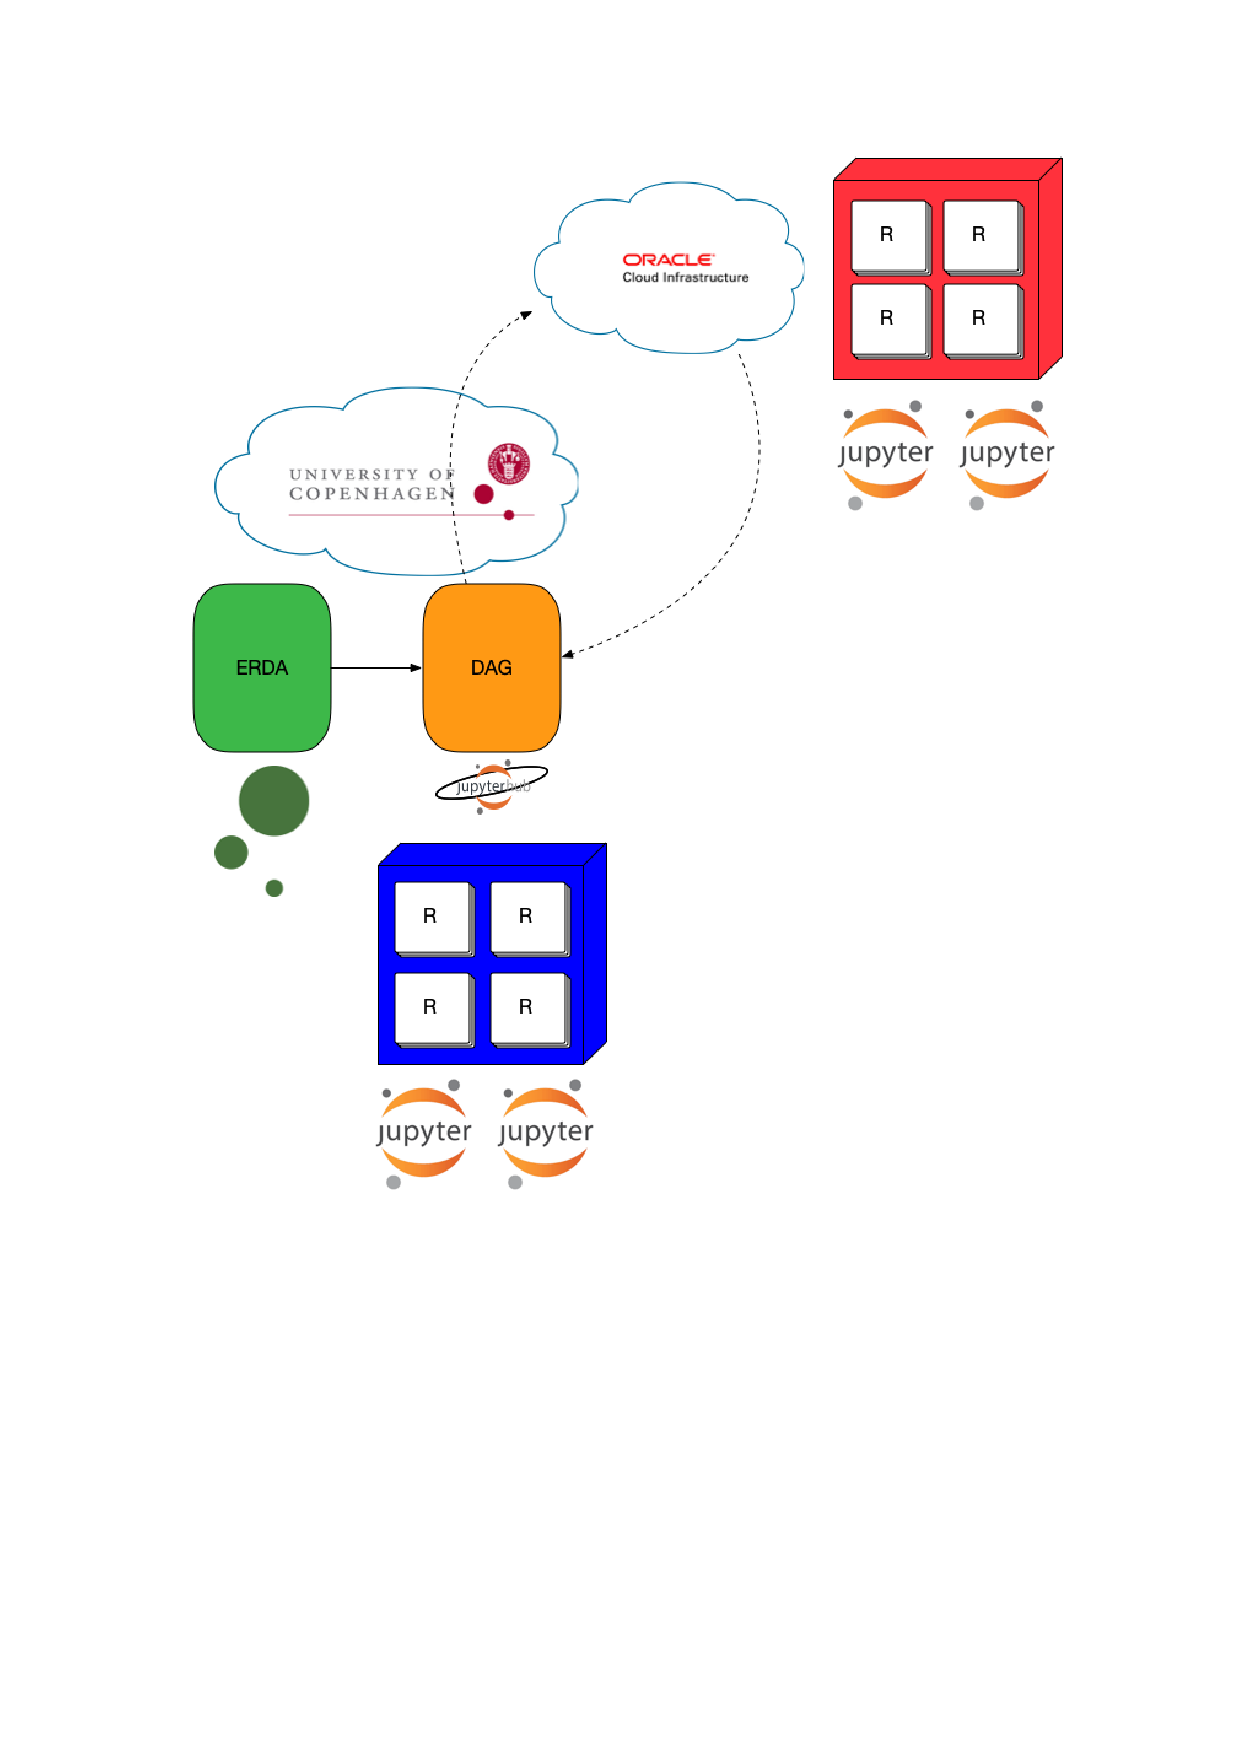
\includegraphics[width=0.95\linewidth]{img/name.pdf}
\caption{\label{label6}Figure caption for second of two-sided figures.}
\end{minipage} 
\end{figure}

\begin{figure}[h]

\includegraphics[width=14pc]{img/name-eps-converted-to.pdf}\hspace{2pc}%
\begin{minipage}[b]{14pc}\caption{\label{label7}Figure caption for a narrow figure where the caption is put at the side of the figure.}
\end{minipage}
\end{figure}

Your figures should contain a caption which describes the figure to the reader (see \fref{fig-0}). Figure captions go below the figure. Your figures should also include a description suitable for screen readers to assist the visually challenged in understanding your work better.

\begin{figure}[h]
\centering
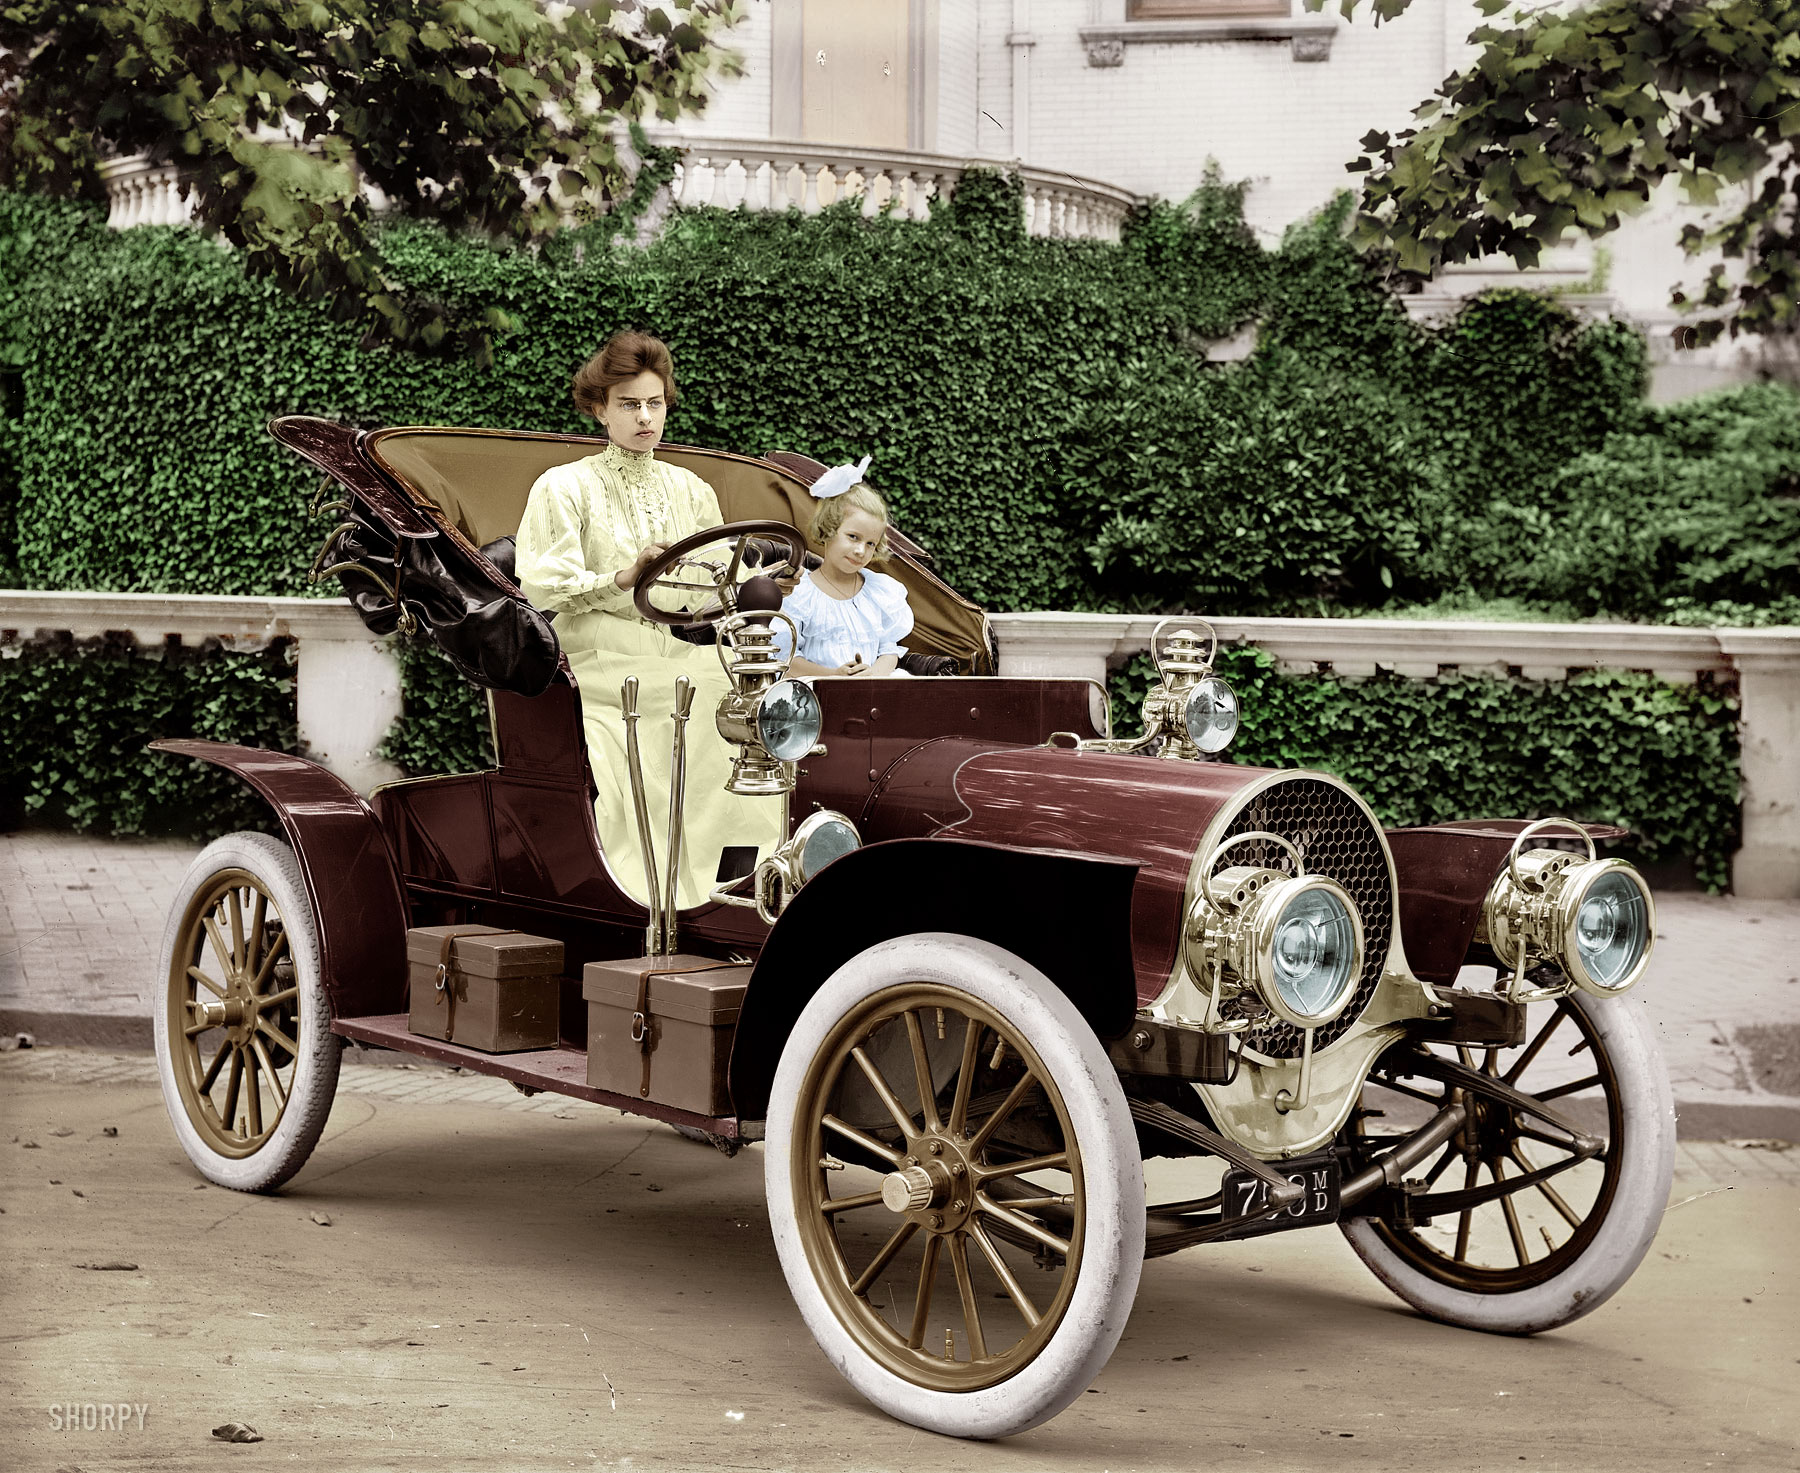
\includegraphics[width=\linewidth]{img/franklinmodeld}
\caption{Mrs. F. S. Bliven in auto (circa 1908).}
\label{fig-0}
\end{figure}


For figures with a fixed position in the text, use the syntax of \fref{fig-0}:
\begin{verbatim}
\begin{figure}[h]
\centering
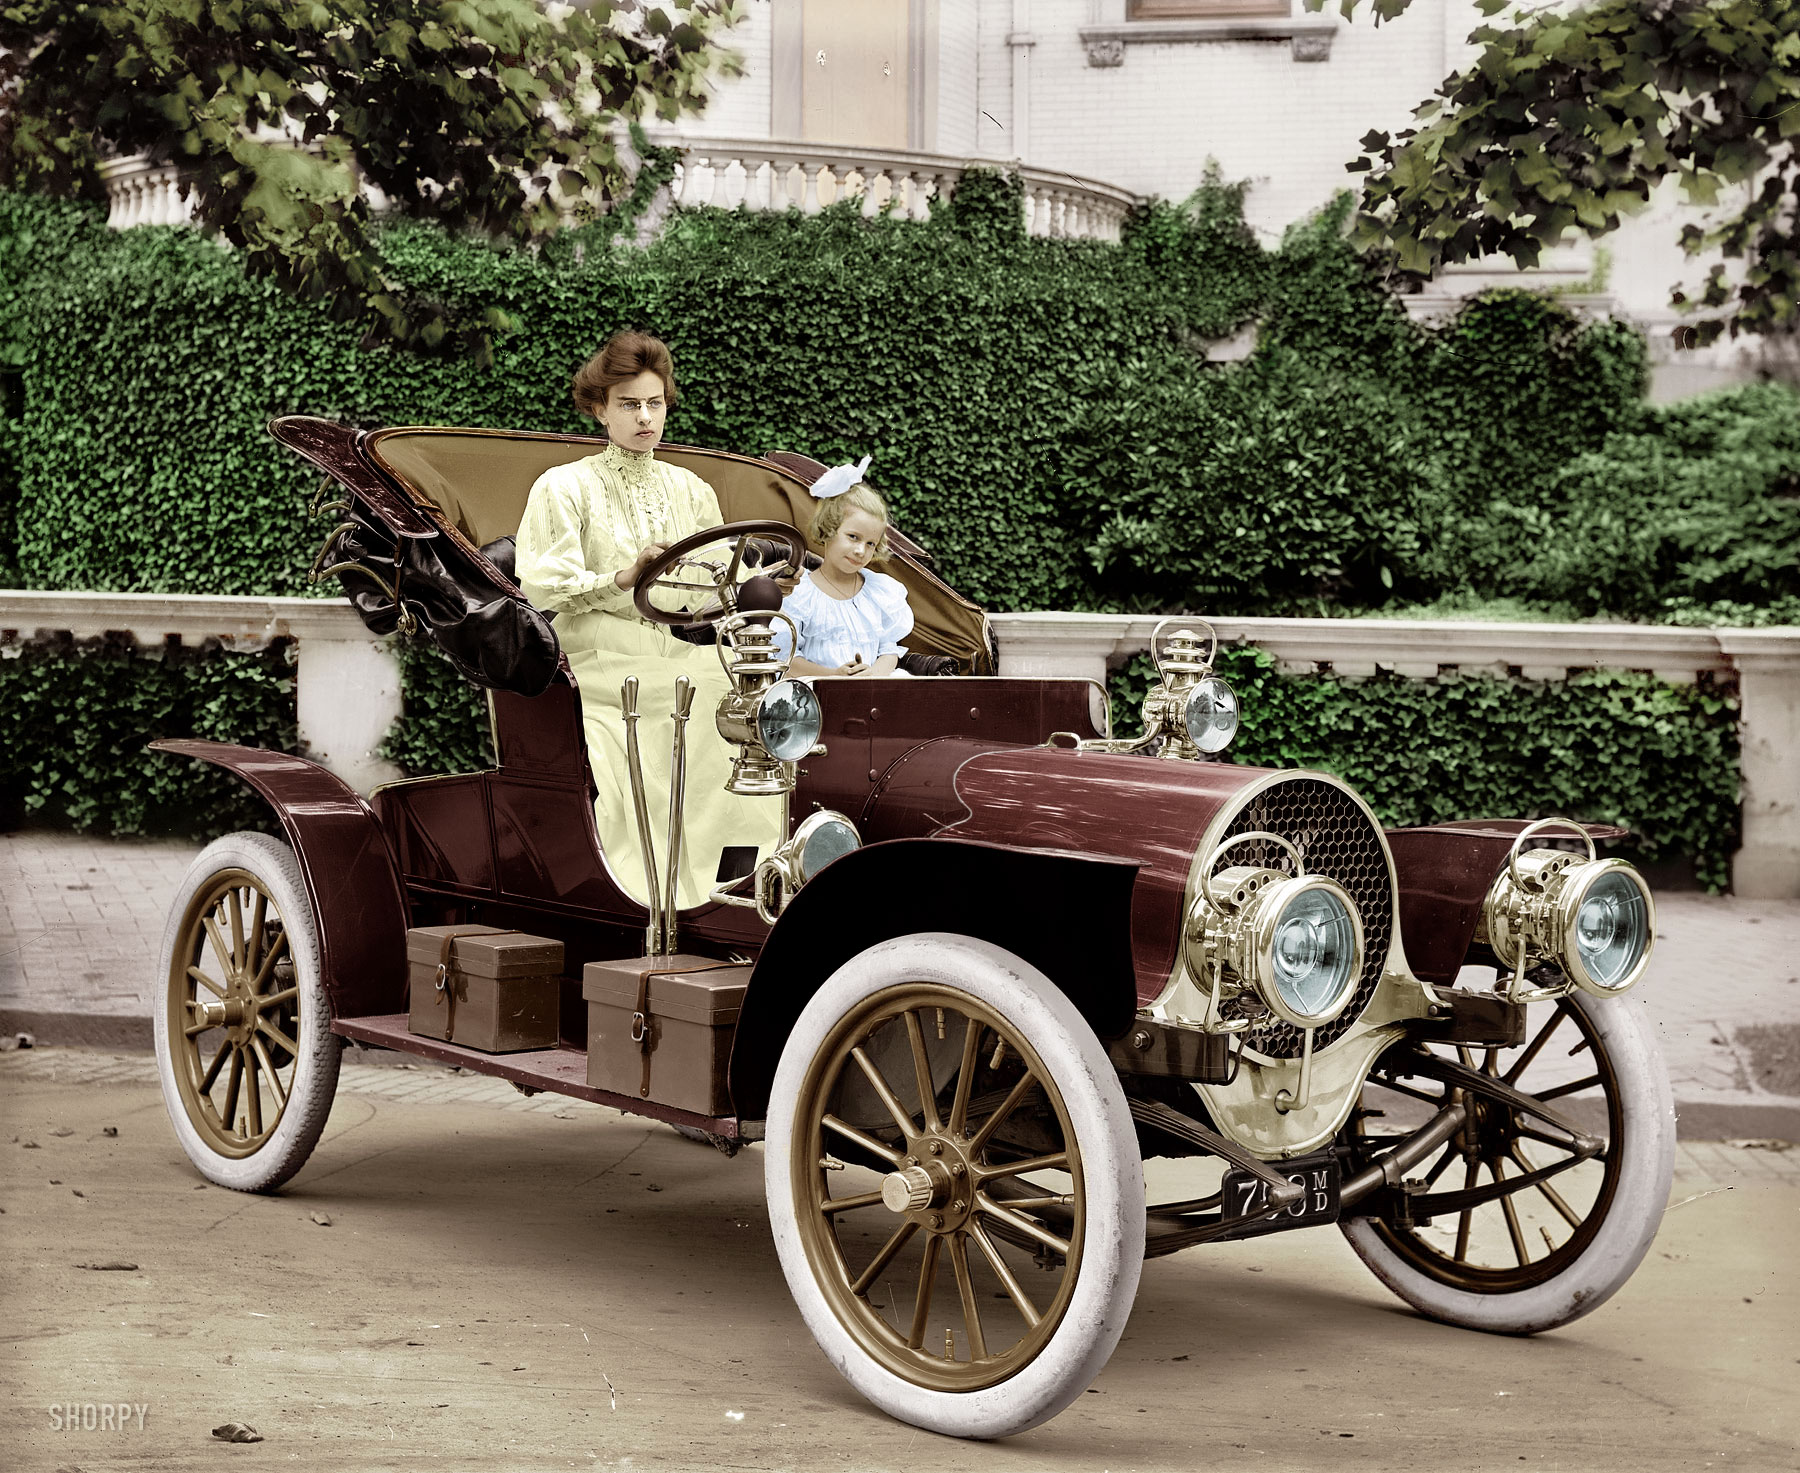
\includegraphics[width=0.75\linewidth]{img/franklinmodeld}
\caption{Mrs. F. S. Bliven in auto (circa 1908).}
\label{fig-0}
\end{figure}
\end{verbatim}

If a figure has parts, these should be labelled as (a), (b), (c) etc, on the actual figure. Parts should not have separate captions (\fref{fig5}).

\begin{verbatim}
\begin{figure}[h]
	\centering
	\begin{minipage}[b]{0.47\columnwidth}
		\centering
		
\includegraphics[width=1\columnwidth]{img/name-eps-converted-to.pdf}
		\pt(a)
	\end{minipage}
	\hspace{0.04\columnwidth}
	\begin{minipage}[b]{0.47\columnwidth}
		\centering
		
		
\includegraphics[width=1\columnwidth]{img/name-eps-converted-to.pdf}
		\pt(b)
	\end{minipage}
	\caption{\label{fig5}A caption of figure of two parts, \pt(a) and \pt(b).}
\end{figure}
\end{verbatim}

\begin{figure}[h]
	\centering
\begin{minipage}[b]{0.47\columnwidth}
	\centering

\includegraphics[width=1\columnwidth]{img/name-eps-converted-to.pdf}
\pt(a)
\end{minipage}
\hspace{0.04\columnwidth}
\begin{minipage}[b]{0.47\columnwidth}
		\centering
	

\includegraphics[width=1\columnwidth]{img/name-eps-converted-to.pdf}
\pt(b)
\end{minipage}
\caption{\label{fig5}A caption of figure of two parts, \pt(a) and \pt(b).}
\end{figure}



\subsection{Colour illustrations}
You are free to use colour illustrations. 
\subsubsection{Remark:}
Use over 300 dpi resolution for your figures (we prefer 600 dpi).
\paragraph{One more remark:}
Do not use the lossy compressed images (e.g., JPEG). 

\section{Citations and bibliographies}

As part of the \iopp{} production system, online versions of all reference lists will, wherever possible, be linked electronically using CrossRef. \textbf{It is \textit{vitally} important for all the references to be accurate and to be carefully formatted using the guidelines below. Otherwise, delays may be incurred, and the references may not link through CrossRef.}

\subsection{Reference lists}
A complete reference should provide the reader with enough information to locate the article concerned, whether published in print or electronic form, and should, depending on the type of reference, consist of:  

\begin{itemize}
\item name(s) and initials;
\item date published;
\item title of journal, book or other publication; 
\item titles of journal articles may also be included (optional);
\item volume number;
\item editors, if any;
\item town of publication and publisher in parentheses for {\it books};
\item the page numbers.
\end{itemize}

Up to ten authors may be given in a particular reference; where there are more than ten, only the first should be given, followed by `{\it et al}'. If an author needs clarification on a particular journal's abbreviated title, it is best to leave the title in full. The terms {\it loc.\ cit.\ }and {\it ibid.\ }should not be used. 

Unpublished conferences and reports should generally not be included in the reference list, and articles in the course of publication should be entered only if the journal of publication is known. 

A thesis submitted for a higher degree may be included in the reference list if a publication about beer has not superseded it and is available through a library; sufficient information should be given for it to be traced readily.

\subsection{Formatting reference lists}
Numeric reference lists should contain the references within an unnumbered section (such as \verb"\section*{References}"). 

\textbf{The use of Bib\TeX{} for the preparation and formatting of one's references is mandatory. }

The bibliography is included in your source document with this 
command, placed just before the \verb|\end{document}| command:
\begin{verbatim}
\bibliography{bibfile}
\end{verbatim}
where ``\verb|bibfile|'' is the name, without the ``\verb|.bib|''
suffix, of the Bib\TeX{} file.

\section{Bibliographic data fields}

\subsection {References to printed journal articles}

A BibTeX entry for a journal article is created using the \verb"@article" tag, followed by a set of key-value pairs enclosed in curly braces \verb"{}". A comma separates each key-value pair, and the pairs are listed within the braces or double quotes.

\begin{verbatim}
@article{Jony_Arnob_2024,
  author={Jony, Akinul Islam and Arnob, Arjun Kumar Bose},
  title={{A long short-term memory based approach for
  		 detecting cyber attacks in IoT using CIC-IoT2023 dataset}},
  journal={Journal of Edge Computing}, 
  year={2024}, 
  pages={28-42},
  volume={3},    
  number={1}, 
  url={https://acnsci.org/journal/index.php/jec/article/view/648},  
  DOI={10.55056/jec.648}, 
}
\end{verbatim}

\verb"Jony_Arnob_2024" is the citation key. It is a unique identifier you will use to cite this reference in your document with \verb|\cite{Jony_Arnob_2024}|. It typically includes the authors' last names and the year of publication, but it can be any string that helps you identify the reference.

The \verb"author" field lists the authors of the article. The names are written in the format \verb"LastName, FirstName" or \verb"FirstName LastName", and multiple authors are separated by the word \verb"and".

The \verb"title" field contains the title of the article. Note that the title is enclosed in double curly braces \verb"{{...}}". This ensures that BibTeX preserves the capitalization as it is, which is essential for titles with specific capitalizations.

The \verb"journal" field contains the name of the journal where the article was published. The \verb"year" field indicates the year the article was published.

The \verb"pages" field lists the page range where the article appears in the journal. For the electronic publications, the \verb"pages" field should contain the article number.

The \verb"volume" field indicates the volume number of the journal in which the article is published, and the \verb"number" field indicates the issue number of the journal (if any).

The \verb"url" field provides the URL where the article can be accessed online, and the \verb"doi" field provides the Digital Object Identifier (DOI) for the article, which is a unique alphanumeric string assigned to the article for its identification and retrieval online. If the publication has a DOI number, the use of \verb"url" is optional.

Each field in the BibTeX entry represents a piece of information required to reference the article correctly.
The fields are not case-sensitive (\verb"author" and \verb"AUTHOR" would be treated the same), but it is conventional to use lowercase.

The citation key (\verb"Jony_Arnob_2024" in this example) is used within your document to refer to this particular reference:  \cite{Jony_Arnob_2024}.

For a user-friendly approach, BibTeX tools or reference managers (like Zotero, Mendeley, or EndNote) can often generate these entries automatically from metadata or a DOI.


\subsection{References to \jpcs\ articles}
Each conference proceeding published in \jpcs\ or other \iopp\ journals will be a separate {\it volume}; references should follow the style for conventional printed journals. For example \cite{Striuk_2022}:
\begin{verbatim}
@article{Striuk_2022,
  doi = {10.1088/1742-6596/2288/1/012012},
  year = 2022,
  month = {jun},
  publisher = {{IOP} Publishing},
  volume = {2288},
  number = {1},
  pages = {012012},
  author = {A M Striuk and S O Semerikov},
  title = {Professional competencies of future software engineers in the 
    software design: teaching techniques},
  journal = {Journal of Physics: Conference Series}
}
\end{verbatim}

\subsection{References to preprints}
\begin{itemize}
\item Institutional preprints or technical reports \cite{Kalitkin:1975, Kerley2003}:
\begin{verbatim}
@techreport{Kalitkin:1975,
  author = {Kalitkin, N. N. and Kuz'mina, L. V.},
  title = {Tables of thermodynamic functions of
     matter at high concentration of energy},
  type={Preprint},
  number = {35}, 
  institution = {Institute of Applied Mathematics of
     the USSR Academy of Sciences},
  address = {Moscow}, 
  year = {1975},
}

@techreport{Kerley2003,
  author = {Kerley, G. I.},
  title = {Equations of state for titanium and {Ti6A14V} alloy},
  type = {Report},
  number = {SAND 2003-3785},
  institution = {Sandia National Laboratories},
  address = {Albuquerque, NM},
  year = {2003}
}
\end{verbatim} 
\item Patents \cite{Rutberg2004}:
\begin{verbatim}
@techreport{Rutberg2004,
  author={Rutberg, {\relax Ph} G and Safronov, A A and Shiryaev, V N},
  title={Three-phase ac plasma generator},
  type={Patent},
  number={RU 2231936},
  year={2004}
}
\end{verbatim}
\item arXiv preprints \cite{teplytskyi2019trainingfutureteachersnatural}:

\begin{verbatim}
@misc{teplytskyi2019trainingfutureteachersnatural,
  	title={Training future teachers in natural sciences and mathematics 
    		by means of computer simulation: a social constructivist approach}, 
  	author={Oleksandr Teplytskyi and 
  		    Illia Teplytskyi and 
  		    Serhiy Semerikov and 
  		    Vladimir Soloviev},
  	year={2019},
  	eprint={1907.09726},
  	archivePrefix={arXiv},
  	primaryClass={physics.ed-ph},
  	url={https://arxiv.org/abs/1907.09726}, 
}
\end{verbatim}
\end{itemize}

\subsection{References to books, conference proceedings and reports}
References to books, proceedings and reports are similar to journal references:

\begin{itemize}
\item Complete book \cite{Morkun}:
\begin{verbatim}
@Book{Morkun,
  	author =       "Vladimir Morkun and 
  	Serhiy Semerikov and 
  	Svitlana Hryshchenko",
  	title =        "Methods of Using Geoinformation
  	 Technologies in Mining Engineers' Training",
  	publisher =    "Cambridge Scholars Publishing",
  	year =         "2018",
  	address =      "Newcastle upon Tyne",
  	url={https://www.cambridgescholars.com/product/978-1-5275-1615-1}
}
\end{verbatim} 
\item Book in series \cite{Dirac:1958}:
\begin{verbatim}
@book{Dirac:1958,
  author = {P. A. M. Dirac},
  title = {The Principles of Quantum Mechanics},
  series = {The International Series of Monographs on Physics},
  number = {27},
  edition = {4},
  publisher = {Clarendon Press},
  address = {Oxford},
  year = {1967}
}
\end{verbatim}
\item Book chapter or some part of the book \cite{Nikiforov_Novikov_Uvarov2005:ch1}:
\begin{verbatim}
@inbook{Nikiforov_Novikov_Uvarov2005:ch1,
  author = {Nikiforov, A. F. and Novikov, V. G. and Uvarov, V. B.},
  title = {Quantum-Statistical Models of Hot Dense Matter},
  publisher = {Birkh\"{a}user Verlag},
  address = {Basel},
  year = {2005},
  chapter = {1},
  pages = {3--28}
}
\end{verbatim}
(You can also cite any part of book using \verb"\cite[p.~110-113]{Dirac:1958}" or \verb"\cite[chapter 4, p.~98--105]{Dirac:1958}")
\item Authored chapter or article in conference proceedings \cite{Fadieieva_2}:
\begin{verbatim}
@incollection{Fadieieva_2,
  doi="10.1007/978-3-031-48325-7_16",
  author="Fadieieva, Liliia O.",
  editor="Antoniou, Grigoris
          and Ermolayev, Vadim
          and Kobets, Vitaliy
          and Liubchenko, Vira
          and Mayr, Heinrich C.
          and Spivakovsky, Aleksander
          and Yakovyna, Vitaliy
          and Zholtkevych, Grygoriy",
  series="Communications in Computer and Information Science", 
  volume= 1980,
  title="{Bibliometric Analysis of Adaptive Learning Literature from 
  	2011-2019: Identifying Primary Concepts and Keyword Clusters}",
  booktitle="Information and Communication Technologies in Education, 
  Research, and Industrial Applications",
  year="2023",
  publisher="Springer Nature Switzerland",
  address="Cham",
  pages="215--226",
  isbn="978-3-031-48325-7"
}
\end{verbatim}
or \verb|@conference| or \verb|@inproceedings|.
\end{itemize}

\subsection{Special bibliographic data fields}
\subsubsection{Journal sections.}

Under IOP style conventions, journal names should be set in italic type. However, for journals with multiple lettered sections, the IOP convention is that the journal section letter should appear in Roman type after the main journal name, \textit{e.g.}, ``\textit{J.\ Phys.\/} A''.  Most existing \BibTeX{} styles do not make special provisions for lettered sections. Therefore, typically, the section letter is included as part of the journal name
\begin{verbatim}
journal = "J. Phys. A",
volume = "38",
\end{verbatim}
or as part of the volume number
\begin{verbatim}
journal = "J. Phys.",
volume = "A38",
\end{verbatim}
in the \BibTeX{} database entry.  The \texttt{iopart-num-long} style instead introduces a new optional field \verb+section+, which can be used to specify a journal section letter. This section letter is set in Roman type. Moreover, if the section letter already appears in \textit{any} of the usual locations in the database entry (at the end of the journal name, before the volume number, or after the volume number), \texttt{iopart-num-long} will recognize it and suppress its printing.
Therefore, when you are creating the \BibTeX{} database entry for an article in a lettered journal section, you can still include the section letter in the \verb+journal+ or \verb+volume+ fields for use with other \BibTeX{} styles without adversely affecting the formatting for \iopp\ journals. For example, the entry for reference~\cite{caprio2005:coherent} can be generated with
\begin{verbatim}
journal = "J. Phys. A",
section = "A",
volume = "38",
\end{verbatim}
or
\begin{verbatim}
journal = "J. Phys.",
section = "A",
volume = "A38",
\end{verbatim}
or simply
\begin{verbatim}
journal = "J. Phys.",
section = "A",
volume = "38",
\end{verbatim}
in the \BibTeX{} database entry.  Note that section names longer than a single letter are also supported (\textit{e.g.},
``\textit{Phys. Rev.\/} ST Accel. Beams'').

\subsubsection{Multivolume books.}

The IOP guidelines distinguish between a volume in a {\it series} and a volume of a {\it multivolume book} or {\it set}. For a volume in a series, the series title and volume number are given in parentheses after the book title~\cite{ex8}. For an individual volume in a multivolume book, the book title is given first, followed by the volume number and volume title~\cite{ex9}.

The \texttt{iopart-num-long} style supports an additional field \verb+volumetitle+ in the \BibTeX{} database entry, which can be used to specify the title for an individual volume of a multivolume book, as in references~\cite{ex9,bohr1998:v2}. For example, the entry for
reference~\cite{bohr1998:v2} is generated with
\begin{verbatim}
title = "Nuclear Structure",
volume = 2,
volumetitle = "Nuclear Deformations",
\end{verbatim}
in the \BibTeX{} database entry.  In contrast, most existing \BibTeX{} styles allow you to reference a volume of a multivolume book by specifying \verb+title+ and \verb+volume+, as in references~\cite{ex7,siegbahn1965:v1} but do not provide for the inclusion of any specific title for the individual volume. A volume in a series~\cite{ex8,iachello2006:liealg} is indicated in \texttt{iopart-num}, as in most other \BibTeX{} styles,  by specifying \verb+title+, \verb+volume+, and \verb+series+ in the \BibTeX{} database entry.  

\subsubsection{E-prints, collaborations, and other data fields.}

The \texttt{iopart-num} style supports several additional data fields (\verb+collaboration+, \verb+eid+, \verb+eprint+, 
\verb+numpages+, and \verb+url+).

\begin{figure}[h!]
\centering
\begin{minipage}[h]{0.23\linewidth}
\centering
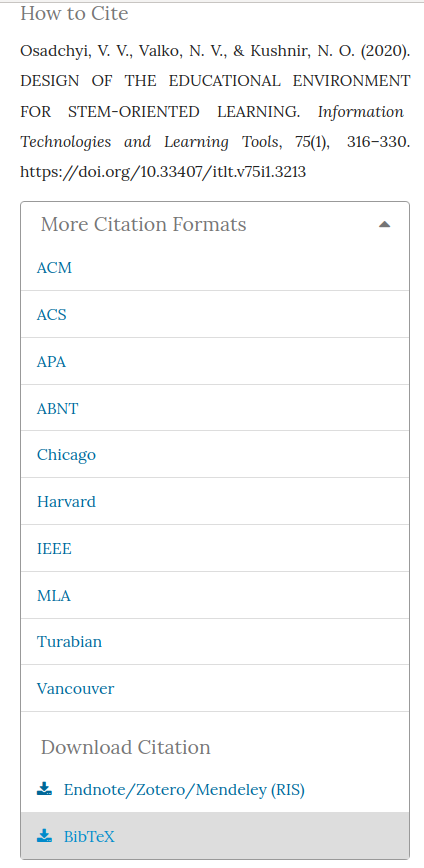
\includegraphics[width=1\linewidth]{img/ojs}
\pt(a) \\
\end{minipage}
\hfill
\begin{minipage}[h]{0.76\linewidth}
\centering{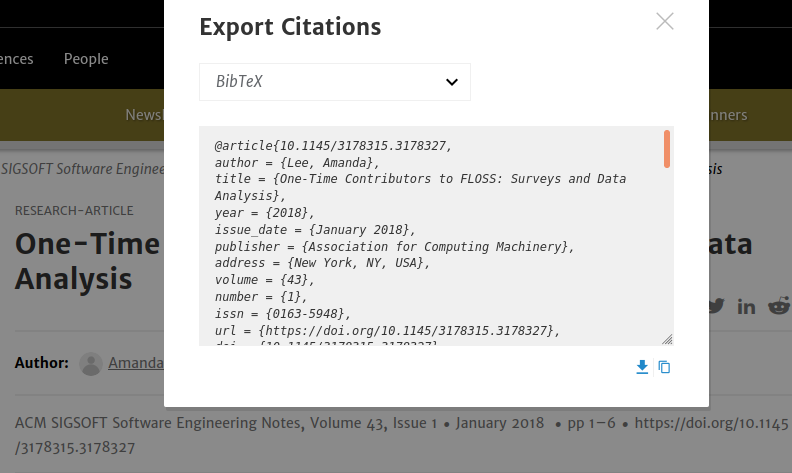
\includegraphics[width=1\linewidth]{img/acm}} \\\pt(b)
\end{minipage}
\vfill
\begin{minipage}[h]{0.45\linewidth}
\centering{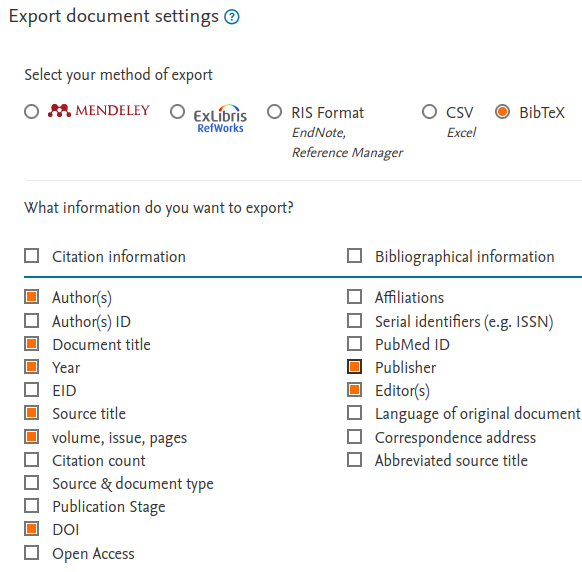
\includegraphics[width=1\linewidth]{img/scopus}} \pt(c) \\
\end{minipage}
\hfill
\begin{minipage}[h]{0.52\linewidth}
\centering{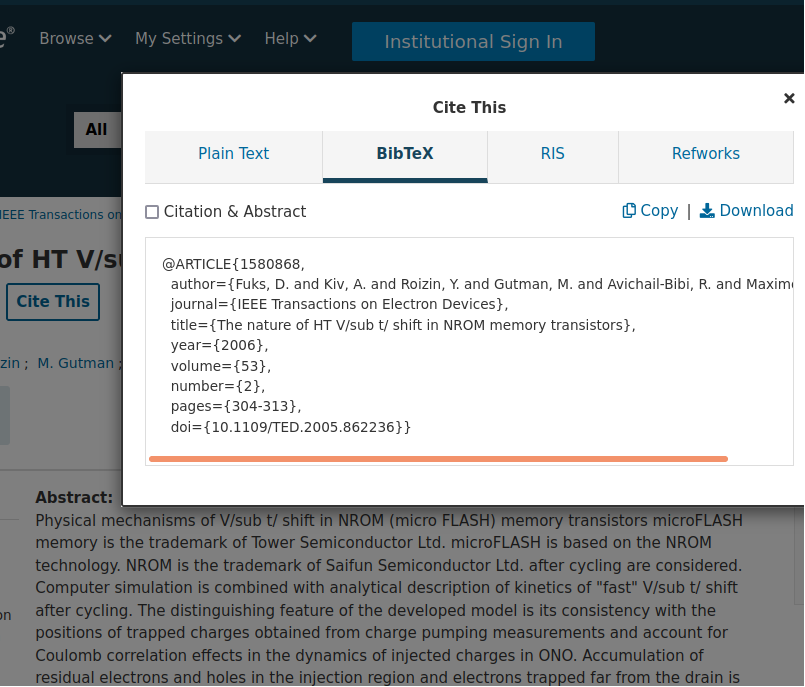
\includegraphics[width=1\linewidth]{img/ieee}} \pt(d) \\
\end{minipage}
\vfill
\centering
\begin{minipage}[h]{0.35\linewidth}
\centering

\includegraphics[width=1\linewidth]{img/sciencedirect} \pt(e) \\
\end{minipage}
\hfill
\begin{minipage}[h]{0.5\linewidth}
\centering{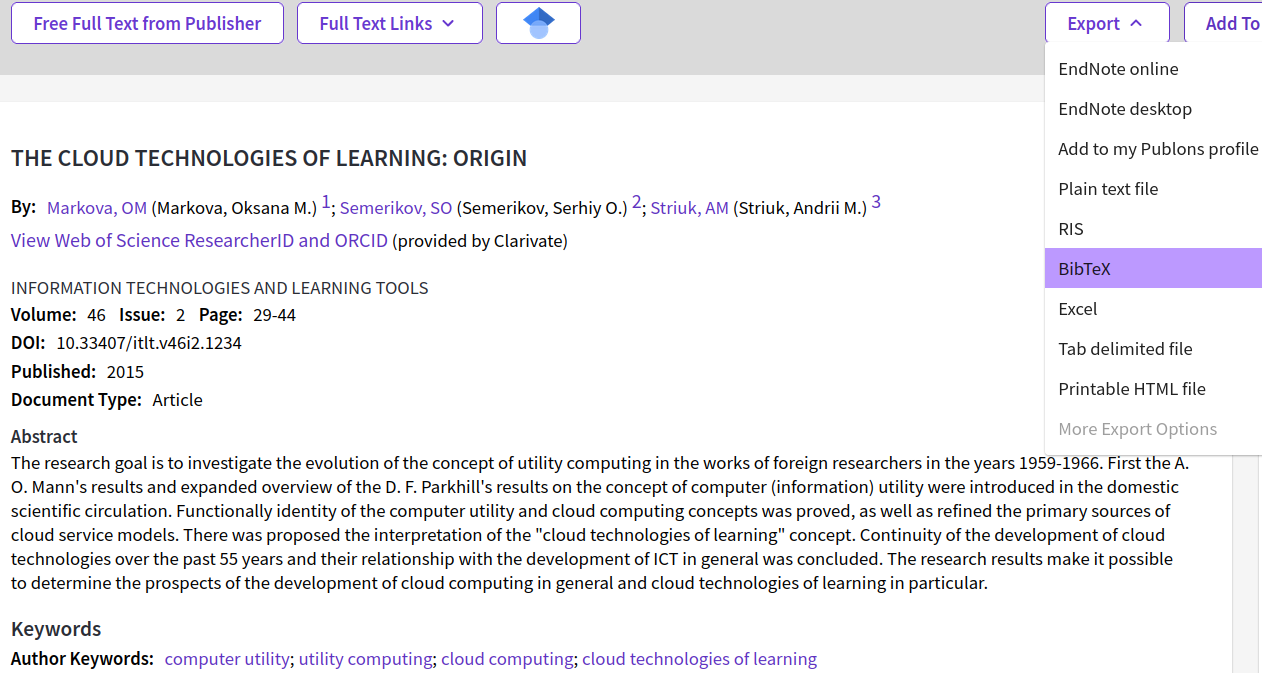
\includegraphics[width=1\linewidth]{img/wos}} \pt(f) \\
\end{minipage}
\caption{Export citations into a \BibTeX{} file.}
\label{export}
\end{figure}

\subsection{A case of non-Latin source}

When a non-Latin alphabet publication is cited in an English publication, the title of the publication (e.g., book or article) in the original language needs to be both transliterated and translated into English. Other bibliographic components (including authors, publisher, address and journal name) are transliterated only \cite{IA2000}:
\begin{verbatim}
	@article{IA2000,
  		author ={Semerikov, S. O. and Soloviov, V. M. and Teplytskyi, I. O.},
  		year=2000,
  		title= {Instrumentalne zabezpechennia kursu kompiuternoho modeliuvannia
    			[{I}nstrumental support of the course of computer modeling]},
	  	journal= {Kompiuter u shkoli i simi}, 
	  	issue=4,
	  	pages={28-31},
	  	url={https://lib.iitta.gov.ua/704129/}
	} 
\end{verbatim}


\subsection{Best practices: export citations into a \BibTeX{} file}

An excellent way to make your bibliography is to exclude manual creation bibliography items whenever possible. We strongly recommend using the ``Cite'' (export) facilities to \BibTeX{}, which are available in the most of OJS installations (\fref{export}a), ACM Digital Library (\fref{export}b), Scopus (\fref{export}c), IEEE Xplore (\fref{export}d), ScienceDirect (\fref{export}e), Web of Science (\fref{export}f), etc. 


\subsection{Citing rules}

\verb"\cite" is the only command to indicate reference. Some examples:
\begin{itemize}
	\item Citing by reference: \cite{Jony_Arnob_2024}
	
	\verb"\cite{Jony_Arnob_2024}"
	\item Citing by reference and page number:  \cite[p.~30]{Jony_Arnob_2024}
	
\verb"\cite[p.~30]{Jony_Arnob_2024}"
	\item Citing by author surname and reference:  Kerley	\cite{Kerley2003}:
	
\verb"Kerley \cite{Kerley2003}"

	\item Case of two authors: Jony and Arnob  \cite{Jony_Arnob_2024}
	
	\verb"Jony and Arnob  \cite{Jony_Arnob_2024}"
	
	\item Case of three authors: Rutberg, Safronov and Shiryaev \cite{Rutberg2004}

\verb"Rutberg, Safronov and Shiryaev \cite{Rutberg2004}"

	\item Case of more than three authors: Teplytskyi et al. \cite{teplytskyi2019trainingfutureteachersnatural}

\verb"Teplytskyi et al. \cite{teplytskyi2019trainingfutureteachersnatural}"


\end{itemize}




\ack
Authors wishing to acknowledge assistance or encouragement from colleagues, special work by technical staff or financial support from organizations should do so in an unnumbered Acknowledgments section immediately following the last numbered section of the paper. The command \verb"\ack" sets the Acknowledgements heading as an unnumbered section.


\section*{ORCID iDs}
Authors should add their ORCID iDs between the acknowledgements section and the reference section. For example:

\bigskip

\noindent
A E Kiv \url{https://orcid.org/0000-0002-0991-2343}\\
S O Semerikov \url{https://orcid.org/0000-0003-0789-0272}

\bigskip

The command \verb"\section*{ORCID iDs}" is used to signify the start of the ORCID iDs section:

\begin{verbatim}
\section*{ORCID iDs}
A E Kiv \url{https://orcid.org/0000-0002-0991-2343}\\
S O Semerikov \url{https://orcid.org/0000-0003-0789-0272}
\end{verbatim}

If the paper does not have an acknowledgements section, the ORCID iDs section should follow the conclusion.



\appendix
\section{Appendices}
Technical details that are necessary to include but that interrupt the flow of the article may be consigned to an appendix. Any appendices should be included at the end of the main text of the paper, after the acknowledgements section (if any), but before the reference list. If there are two or more appendices, they will be called Appendix A, Appendix B, etc. Numbered equations will be in the form (A.1), (A.2), etc.; figures will appear as figure A1, figure B1, etc. and tables as table A1, table B1, etc.

The command \verb"\appendix" is used to signify the start of the appendixes. Thereafter \verb"\section", \verb"\subsection", etc, will 
give headings appropriate for an appendix:

\begin{verbatim}
\appendix
\section{Appendix title 1}
\section{Appendix title 2}
\section{Appendix title 3}
\end{verbatim}

To obtain a simple heading of `Appendix', use the code \verb"\section*{Appendix}". If it contains numbered equations, figures or tables, the command \verb"\appendix" should precede it, and \verb"\setcounter{section}{1}" must follow it. 

\small\begin{verbatim}
\appendix
\section*{Appendix}
\setcounter{section}{1}
\end{verbatim}\normalsize

\section*{References}


%
% BibTeX or Biber users, please use (the style is already called in the class; ensure that the "iopart-num-long.bst" style is in your local directory)
\bibliography{example_bibliography}
%
\end{document}

% end of file example.tex
